\chapter{Governing Equations}
\label{chap:landice-mobal}

% ===============================
% ===============================
%\section{Conservation Equations}
% ===============================
% ===============================

The ``dynamical core'' of the the MALI ice sheet model solves the governing equations expressing the conservation of momentum, mass, and energy.   

\section{Conservation of Momentum}
\label{sec:consmom}

Treating glacier ice as an incompressible fluid in a low-Reynolds number flow,
%for which acceleration is negligible, 
the conservation of momentum in a Cartesian reference frame is expressed by the Stokes-flow equations, for which the gravitational-driving stress is balanced by gradients in the viscous stress tensor, $\sigma_{ij}$:
\begin{equation}
\frac{\partial \sigma_{ij}}{\partial x_{j}} + \rho g ~=~0, ~~i,j=1,2,3
\label{eq:mobal}
\end{equation}
\noindent
where $x_i$ is the coordinate vector, $\rho$ is the density of ice, and $g=$ is acceleration due to gravity\footnote{In Equation \ref{eq:mobal} and elsewhere we use indicial notation, with summation over repeat indices.}.

Deformation results from the deviatoric stress, $\tau_{ ij}$, which relates to the full stress tensor as
\begin{equation}
\tau_{ ij} ~ = ~ \sigma _{ ij} ~ - ~{\frac{ 1}{ 3}} \sigma _{ kk} \delta _{ ij},
\label{eq:mobaldevia}
\end{equation}
\noindent
for which ${-\frac{1}{ 3}} \sigma _{ kk}$ is the mean compressive stress and $\delta_{ ij}$ is the Kroneker delta (or the identity tensor). 
Stress and strain rate are related through the constitutive relation,
\begin{equation}
\tau_{ij}~=~2 \eta_{e} \dot{\epsilon}_{ij},
\label{eq:tauij}
\end{equation}
where $\dot{\epsilon_{ij}}$ is the strain-rate tensor and $\eta_{e}$ is the ``effective'', non-Newtonian ice viscosity given by Nye's generalization of Glen's flow law \citep{Glen1955}, 
\begin{equation}
\eta_{e}~=~\gamma A^{-\frac{1}{n}} \dot{\epsilon}_{e}^{\frac{1-n}{n}}.
\label{eq:mobalGlen}
\end{equation}
In Equation \ref{eq:mobalGlen}, $A$ is a temperature dependent rate factor, $n$ is an exponent commonly taken as 3 for polycrystalline glacier ice, and $\gamma$ is an ice ``stiffness'' factor (inverse enhancement factor) commonly used to account for other impacts on ice rheology, such as impurities or crystal anisotropy (see also Section \ref{sec:optimInit}). The effective strain rate $\dot{\epsilon}_{e}$  is given by the second invariant of the strain-rate tensor,
\begin{equation}
\dot{\epsilon}_{e}=\left(\frac{1}{2}\dot{\epsilon}_{ij}\dot{\epsilon}_{ij}\right)^{\frac{1}{2}},
\label{eq:effstrain}
\end{equation}
The strain rate tensor is defined by gradients in the components of the ice velocity vector $u_i$:
\begin{equation}
\dot{\epsilon}_{ij}~= \frac{1}{2}\left( \frac{ \partial u_{i}}{\partial x_{j}} + \frac{ \partial u_{j}}{\partial x_{i}}\right), ~~i,j = 1,2,3.
\label{eq:mobalstrainrate}
\end{equation}
Finally, the rate-factor $A$ follows an Arrhenius relationship
\begin{equation}
A\left( T^{*}\right)~=~A_{o}e^{-Q_a/RT^{*}},
\label{eq:mobalA}
\end{equation}
\noindent
in which $A_{o}$ is a constant, $(T^{*})$ is the absolute temperature (i.e., corrected for the dependence of melt temperature on ice pressure),
$Q_a$ is the activation energy for crystal creep, and $R$ is the gas constant.
%, and $E$ is an enhancement factor commonly used to account for other impacts on ice rheology, such as impurities or crystal anisotropy. 
%tuning parameter, which can be used to account for the effects of impurities and anisotropic ice fabrics. 

Boundary conditions required for the solution of Eq. \ref{eq:mobal} depend on the form of reduced-order approximation applied and are discussed further below.
%include a free upper surface, no slip or continuity of basal tractions at the ice-bed interface (depending on frozen or thawed basal conditions, respectively), and hydrostatic ocean pressure against lateral boundaries where terminating in the ocean. The specific form of these boundary conditions depends on which reduced-order approximation to the Stokes equations is assumed, which we discuss further below.  

% ===============================
\section{Reduced-order Equations}
\label{sec:consmomred}

Ice sheet models solve Eq. \ref{eq:mobal}-\ref{eq:mobalA} with varying degrees of complexity in terms of the tensor components in Eq. \ref{eq:mobal}-\ref{eq:mobalstrainrate} that are accounted for or omitted, based on geometric scaling arguments. Because ice sheets are inherently ``thin'' -- their widths are several orders of magnitude larger than their thickness -- reduced-order approximations of the full momentum balance are often appropriate \citep[see, e.g.,][]{Dukowicz2010,Schoof2013} and, importantly, can often result in considerable computational cost savings. Here, we employ two such approximations, a first-order-accurate ``Blatter-Pattyn'' approximation and a zero-order, ``shallow-ice approximation'' as described in more detail in the following sections.

% ===============================
\subsection{First-Order Velocity Solver and Coupling}
\label{sec:foMomBal}

Ice sheets typically have a small aspect ratio, small surface and bed slopes, and vertical pressure distributions that are very nearly hydrostatic. These characteristics imply that reduced-order approximations of the Stokes momentum balance may apply over large areas of the ice sheets, potentially allowing for significant computational savings. Formal derivations involve non-dimensionalizing the Stokes momentum balance and introducing a geometric scaling factor, $\delta=H/L$, where $H$ and $L$ represent characteristic vertical and horizontal length scales (often taken as the ice thickness and the ice sheet span), respectively. Upon conducting an asymptotic expansion, reduced-order models with a chosen degree of accuracy (relative to the original Stokes flow equations) can be derived by retaining terms of the appropriate order in $\delta$. For example, the first-order accurate Stokes approximation is arrived at by retaining terms of $\mathcal{O}(\delta^1)$ and lower (The reader is referred to \cite{Schoof2010} and \cite{Dukowicz2010} for additional discussion\footnote{In practice, additional scaling parameters describing the ratio of deformation to sliding velocity may also be introduced.}). 

Using the notation  of \cite{perego2012} and \citet{tezaur2015a}
\footnote{Vectors and tensors are given in bold rather than using indices.  Note that, in a slight abuse of notation, we have switched from using $x_1$, $x_2$, $x_3$ to denote the three coordinate directions to $x$, $y$, $z$.}, 
the first-order accurate Stokes approximation \citep[also referred to as the ``Blatter-Pattyn'' approximation, see][]{BLATTER1995,pattyn2003} is expressed through the following system of PDEs, 
\begin{equation} \label{eq:foStokes}
\left\{
\begin{array}{rcl} -\nabla \cdot (2 \eta_f \dot{\boldsymbol{\epsilon}}_1) + \rho g
\frac{\partial s}{\partial x}&=&0, \\
-\nabla \cdot (2 \eta_f \dot{\boldsymbol{\epsilon}}_2) +\rho g
\frac{\partial s}{\partial y} &=& 0, \\
\end{array}\right.
\end{equation}
where $\nabla \cdot $ is the divergence operator, $s\equiv s(x,y)$ represents the ice sheet upper surface, and the vectors $\dot{\boldsymbol{\epsilon}}_1$ and $\dot{\boldsymbol{\epsilon}}_2$ are given by 
\begin{equation}
\dot{\boldsymbol{\epsilon}}_1 = \left(\begin{array}{ccc}
2\dot{\epsilon}_{xx} + \dot{\epsilon}_{yy}, &\dot{\epsilon}_{xy},&
\dot{\epsilon}_{xz}\end{array}\right)^T,
\end{equation}
and
\begin{equation}
\dot{\boldsymbol{\epsilon}}_2 = \left(
\begin{array}{ccc}\dot{\epsilon}_{xy}, &
\dot{\epsilon}_{xx} + 2\dot{\epsilon}_{yy}, &\dot{\epsilon}_{yz}
\end{array}\right)^T.
\end{equation}
Akin to Equations \ref{eq:mobalGlen} and \ref{eq:effstrain}, $\eta_f$ in Equation \ref{eq:foStokes} represents the effective viscosity but for the case of the first-order stress balance with an effective-strain rate is given by
\begin{equation} \label{eq:effStrain2}
\dot{\epsilon}_e \equiv \left( \dot{\epsilon}_{xx}^2 +
\dot{\epsilon}_{yy}^2 + \dot{\epsilon}_{xx} \dot{\epsilon}_{yy} +
\dot{\epsilon}_{xy}^2 + \dot{\epsilon}_{xz}^2 +
\dot{\epsilon}_{yz}^2 \right)^\frac{1}{2},
\end{equation}
rather than by Equation \ref{eq:effstrain}, and with individual strain rate terms given by,
\begin{equation} \label{eq:epsilonij}
\dot{\epsilon}_{xx} = \frac{\partial u}{\partial x}, \hspace{0.5cm} 
\dot{\epsilon}_{yy} = \frac{\partial v}{\partial y}, \hspace{0.5cm}
\dot{\epsilon}_{xy} = \frac{1}{2}\left(\frac{\partial u}{\partial y} + \frac{\partial v}{\partial x} \right), \hspace{0.5cm}
\dot{\epsilon}_{xz} = \frac{1}{2} \frac{\partial u}{\partial z}, \hspace{0.5cm} 
\dot{\epsilon}_{yz} = \frac{1}{2} \frac{\partial v}{\partial z}.
\end{equation}

At the upper surface, a stress-free boundary condition is applied, 
\begin{equation} \label{eq:stressFreeBC}
\dot{\boldsymbol{\epsilon}}_1 \cdot \mathbf{n} = \dot{\boldsymbol{\epsilon}}_2 \cdot \mathbf{n} = 0,% \hspace{0.5cm}, \text{on } z=s(x,y),%\Gamma_s.
\end{equation}
with $\mathbf{n}$ the outward normal vector at the ice sheet surface, $z=s(x,y)$. At the bed, $z=b(x,y)$, we apply no slip or continuity of basal tractions (``sliding''),
\begin{equation} \label{eq:basalBC}
%\left\{ 
\begin{array}{ll}
u = v = 0, & \text{no slip} \\% \Gamma_0 \\
2\mu \dot{\boldsymbol{\epsilon}}_1 \cdot \mathbf{n} + \beta u^{m} = 0, \hspace{0.2cm} 2 \mu \dot{\boldsymbol{\epsilon}}_2 \cdot \mathbf{n} + \beta v^{m} = 0, & \text{sliding,} \\% \Gamma_{\beta}.
\end{array}
%\right.
\end{equation}
where $\beta$ is a linear-friction parameter and $m\geq1$. In most applications we set $m = 1$ (see also Section \ref{sec:sgh-coupling}).   

On lateral boundaries, a stress boundary condition is applied, 
\begin{equation}\label{eq:oceanBC}
%\left\{
\begin{array}{ll}
2 \mu \dot{\boldsymbol{\epsilon}}_i \cdot \mathbf{n} -\rho g (s-z)\mathbf{n} = \rho_o g \max(z,0) \mathbf{n}, %& \text{on }\Gamma_l,
\end{array}
%\right.
\end{equation}
where $\rho_o$ is the density of ocean water and $\mathbf{n}$ the outward normal vector to the lateral boundary (i.e., parallel to the $(x,y)$ plane), so that lateral boundaries above sea level are effectively stress free and lateral boundaries submerged within the ocean experience hydrostatic pressure due to the overlying column of ocean water. 
%{\color{blue}[Looks good to me. Should we add here other boundary conditions? Schoof etc..]}

We solve these equations using the Albany-LI momentum balance solver, which is built using the Albany and Trilinos software libraries discussed above. The mathematical formulation, discretization, solution methods, verification, and scaling of Albany-LI are discussed in detail in \cite{tezaur2015a}. 
Albany-LI implements a classic finite element discretization of the first-order approximation. At the grounding line, the basal friction coefficient $\beta$ can abruptly drop to zero within an element of the mesh. This discontinuity is resolved by using an higher-order Gauss quadrature rule on elements containing the grounding line, which corresponds to the  sub-element parametrization \emph{SEP3} proposed in \cite{Seroussi2014a}.
Additional exploration of solver scalability and demonstrations of solver robustness on large scale, high-resolution, realistic problems are discussed in \cite{tezaur2015b}. 
The efficiency and robustness of nonlinear solvers are achieved using a combination of the Newton method (damped with a line search strategy when needed) and of a parameter continuation algorithm for the numerical regularization of the viscosity. 
The scalability of linear solvers is obtained using a multilevel preconditioner (see \cite{Tuminaro2016}) specifically designed to target shallow problems characterized by meshes extruded in the vertical dimension, like those found in ice sheet modeling.
The preconditioner has been demonstrated to be particularly effective and robust even in the presence of ice shelves that typically lead to highly ill-conditioned linear systems. Because the momentum balance solver is $\geq95\%$ of the cost of a typical forward model time step, the model performance reported on in \cite{tezaur2015a,tezaur2015b} and \cite{Tuminaro2016} is generally representative of overall MALI performance.   
% The Albany-LI velocity solver deployed within the Community Ice Sheet Model
% was used to demonstrate a validation framework for the Greenland Ice Sheet,
% including a 350 kyr model spinup at 1 km resolution \citep{Price2017}.

The Albany-LI first-order velocity solver written in C++ is coupled to MPAS written in Fortran using an interface layer.
Albany uses a three-dimensional mesh extruded from a basal triangulation and composed of prisms or tetrahedra (see \cite{tezaur2015a}). 
When coupled to MPAS, the basal triangulation is the part of the Delaunay triangulation, dual to an MPAS Voronoi mesh, that contains active ice and it is generated by the interface.
Bed topography, ice lower surface, ice thickness, basal friction coefficient ($\beta$), and three-dimensional ice temperature,
all at cell centers (Table \ref{table:meshes}), are passed from MPAS to Albany.
Optionally, Dirichlet velocity boundary conditions can also be passed.
After the velocity solve is complete, Albany returns the $x$ and $y$ components of velocity at each cell center and blue layer interfaces, the normal component of velocity at each cell edge and blue layer interfaces, and viscous dissipation at blue each cell vertex and layer midpoints.
%Because MPAS uses a Voronoi grid for finite volume methods while Albany uses the subset of the dual Delaunay T=triangulation that contains active ice for finite element methods, the interface code must also generate the finite element triangulation to be used.

The interface code defines the lateral boundary conditions on the finite element mesh that Albany will use.
Lateral boundaries in Albany are applied at cell centers (triangle nodes) that do not contain dynamic ice on the MPAS mesh and that are adjacent to the last cell of the MPAS mesh that does contain dynamic ice.
This one element extension is required to support calculation of normal velocity on edges ($u_n$) required for advection 
of ice out of the final cell containing dynamic ice (Figure \ref{fig:mesh-bc}).
The interface identifies three types of lateral boundaries for the first-order velocity solve: terrestrial, floating marine, and grounded marine.
Terrestrial margins are defined by bed topography above sea level.  
At these boundary nodes, ice thickness is set to a small ice minimum thickness value ($\epsilon=1$ m).
Floating marine margin triangle nodes are defined as neighboring one or more triangle edges that satisfy the hydrostatic floatation criterion.
At these boundary nodes, we need to ensure the existence of a realistic calving front geometry, 
so we set ice thickness to the minimum of thickness at neighboring cells with ice.
Grounded marine margins are defined as locations where the bed topography is below sea level, 
but no adjacent triangle edges satisfy the floatation criterion.
At these boundary nodes, we apply a small floating extension with thickness $\epsilon$.
For all three boundary types, ice temperature is averaged from the neighboring locations containing ice.


%\begin{table*}[t]
%\caption{Correspondence between the MPAS Voronoi tesselation and its dual Delaunay triangulation used by Albany.
%Key MALI model variables that are natively found at each location are listed.  Note that variables are interpolated from 
%one location to another as required for various calculations.
%}
%\begin{tabular}{lll}
%\tophline
%Voronoi tesselation & Delaunay triangulation & Variables\\
%\middlehline
%cell center & triangle node   & $H, T, u, v$, $\Phi$ (MPAS) \\
%cell edge   & triangle edge   & $u_n$ (for advection) \\
%cell vertex & triangle center & $\Phi$ (Albany)\\
%\bottomhline
%\end{tabular}
%\belowtable{} % Table Footnotes
%\label{table:meshes}
%\end{table*}


\begin{figure}[t]
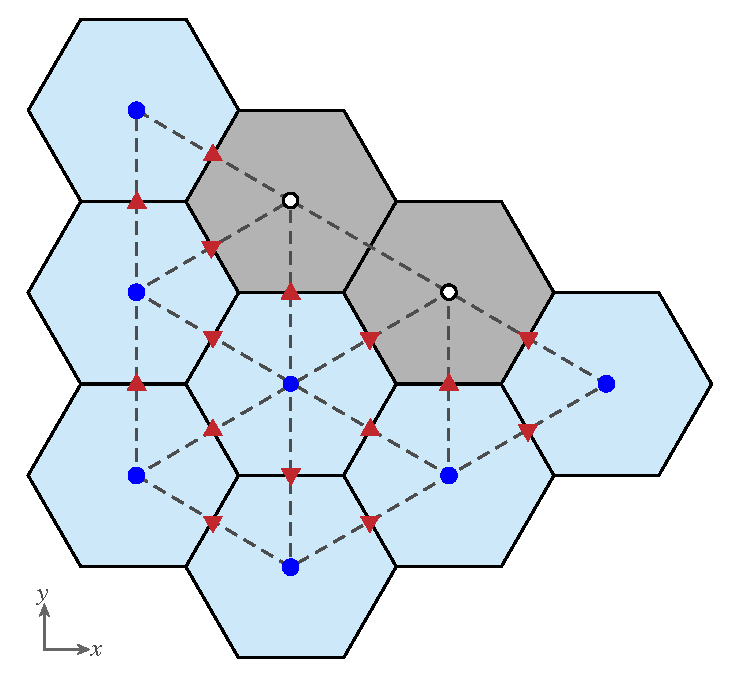
\includegraphics[width=7.0cm]{landice/figures/mpas_grid_albany_bc.pdf}
\caption{Correspondence between MPAS and Albany meshes and application of boundary conditions for the first-order velocity solver.
Solid black lines are cells on the Voronoi mesh and dashed gray lines are triangles on the Delaunay Triangulation.
Light blue Voronoi cells contain dynamic ice and gray cells do not.  
Dark blue circles are Albany triangle nodes that use variable values directly from the co-located MPAS cell centers.
White circles are extended node locations that receive variable values as described in the text based on whether they are terrestrial, floating marine, or grounded marine locations.
Red triangles indicate Voronoi cell edges on which velocities ($u_n$) are required for advection.
}
\label{fig:mesh-bc}
\end{figure}


% ===============================
\subsection{Shallow-Ice Approximation Velocity Solver}
\label{sec:zoMomBal} % zero-order mom. bal.

A similar procedure to that described above for the first-order accurate Stokes approximation can be used to derive the so-called ``shallow-ice approximation'' (SIA) \citep{Hutter1983, Fowler1978a, Morland1980,payne2000}, in this case by retaining only terms of $\mathcal{O}(\delta^0)$. In the case of the SIA, the local gravitational driving stress is everywhere balanced by the local basal traction and the horizontal velocity as a function of depth is simply the superposition of the local basal sliding velocity and the integral of the vertical shear from the ice base to that depth:
\begin{equation}
%\langle u,v \rangle = -2(\rho g)^{n} \left(\int_{b}^{z} A s (h-s)^{n} dz \right) |\nabla h|^{n-1} \nabla h + u_b
\boldsymbol{u} = -2(\rho g)^{n} \left(\int_{b}^{z} A (s-z)^{n} dz \right) |\nabla s|^{n-1} \nabla s + \boldsymbol{u_b}
\label{eq:SIA1}
\end{equation}
where $b$ is the bed elevation and $\vec{u_b}$ is the sliding velocity. 
%{\color{red} \textbf{Matt, please check above -- I changed the $u$ and $u_b$ to be in vector format, as above.}}

SIA ice sheet models typically combine the momentum and mass balance equations to evolve the ice geometry directly in the form of a depth-integrated, two-dimensional diffusion problem \citep{Hindmarsh1996,payne2000}.
However we implement the SIA as an explicit velocity solver that can be enabled in place of the more accurate first order solver,
while keeping the rest of the model identical.
The purpose of the SIA velocity solver is primarily for rapid testing, so the less efficient explicit implementation  of Eq. \ref{eq:SIA1} is not a concern. 

We implement Eq. \ref{eq:SIA1} in sigma coordinates on cell edges, where
we only require the normal component of velocity, $u_n$:
\begin{equation}
u_n = -2(\rho g)^{n} H^{n+1} |\nabla s|^{n-1} \frac{ds}{dx_n} \int_{1}^{\sigma} A \sigma^n d\sigma + u_{b_n}
\label{eq:SIA2}
\end{equation}
where $x_n$ is the normal direction to a given edge and $u_{b_n}$ is sliding velocity in the normal direction to the edge.
We average $A$ and $H$ from cell centers to cell edges.  
$\frac{ds}{dx_n}$ is calculated as the difference in surface elevation between the 
two cells that neighbor a given edge divided by the distance between the cell centers;
on a Voronoi grid, cells edges are midway between cell centers by definition.
The surface slope component tangent to an edge (required to complete the calculation of $\nabla s$) is calculated by first interpolating surface elevation from cell centers to vertices. 


% ===============================
\section{Conservation of Mass}
\label{sec:consMass}

Conservation of mass is used to conduct ice sheet mass transport and evolution.
Assuming constant density to write conservation of mass in volume form, 
the equation relates ice thickness change to the divergence of mass and sources and sinks:
\begin{equation}
\frac{\partial H}{\partial t} + \nabla \cdot H \mathbf{\bar{u}} = \dot{a} + \dot{b},
\label{eq:mass}
\end{equation}
where $H$ is ice thickness, $t$ is time, $\mathbf{\bar{u}}$ is depth-averaged velocity,
$\dot{a}$ is surface mass balance, and $\dot{b}$ is basal mass balance.
Both $\dot{a}$ and $\dot{b}$ are positive for ablation and negative for accumulation.

Eq. \ref{eq:mass} is used to update thickness in each grid cell on each time step using 
a forward Euler, fully explicit time evolution scheme.
Eq. \ref{eq:mass} is implemented using a finite volume method, such that fluxes are calculated for
each edge of each cell to calculate $\nabla \cdot H \mathbf{\bar{u}}$.
Specifically, we use a first-order upwind method that applies the normal velocity on each edge ($u_n$) and 
an upwind value of cell centered ice thickness.
Note that with the First Order velocity solver, normal velocity is interpolated from cell centers to
edges using the finite element basis functions in Albany.  
In the shallow ice approximation velocity solver, normal velocity is calculated natively at edges.
MPAS Framework includes a higher-order flux-corrected transport scheme \citep{Ringler2013} 
for which we have performed some initial testing, but is not routinely used in the Land Ice core at this time.

Tracers are advected layer by layer with a similar equation:
\begin{equation}
\frac{\partial (Q_t l)}{\partial t} + \nabla \cdot \left( Q_t l \mathbf{\bar{u}} \right)= \dot{S}
\label{eq:tracers}
\end{equation}
where $Q_t$ is a tracer quantity (e.g., temperature -- see below), $l$ is layer thickness, and $\dot{S}$ represents any tracer sources or sinks.
While any number of tracers can be included in the model, the only one to be considered here is temperature,
due to its important effect on ice rheology through Eq. \ref{eq:mobalA}
and will be discussed further in the following section. 

Because we employ a sigma vertical coordinate system with fixed layer fractions,
after Eqs. \ref{eq:mass} and \ref{eq:tracers} are applied, a vertical remapping operation is required.
Overlaps between the newly calculated layers and the target sigma layers are calculated for each grid cell.
Assuming uniform values within each layer, mass, energy, and other tracers are transferred between layers
based on these overlaps to restore the prescribed sigma layers while conserving mass and energy.

% ===============================
\section{Conservation of Energy}
\label{sec:consEnergy}

Conservation of energy is expressed through the three-dimensional, advective-diffusive heat equation: 
%\textit{SP: I think that for now, we should leave out the enthalpy formulation since we don't have a good description of that in hand already and it's not yet been tested.}
\begin{equation}
   \label{eq:tempEvolFull}
  \frac{\partial T}{\partial t} = 
  {\frac{1}{\rho c}}{\frac{\partial }{\partial x_{ i}}}\left(k{\frac{\partial T}{\partial x_{ i}}}\right) - {u_{ i}}{\frac{\partial T}{\partial x_{ i}}} + \frac{\Phi}{\rho c},
\end{equation}
with thermal conductivity $k$ and heat capacity $c$. In Equation \ref{eq:tempEvolFull}, the rate of temperature change (left-hand side) is balanced by diffusive, advective, and internal (viscous dissipation -- see Equation \ref{eq:viscDisspTerm} for $\Phi$) source terms (first, second, and third terms on the right-hand side, respectively). 
In MALI we solve an approximation of Equation \ref{eq:tempEvolFull}, 
\begin{equation}
  \label{eq:tempEvolApprox}
  \frac{\partial T}{\partial t} = 
  {\frac{k}{\rho c}}{\frac{\partial^{2} T}{\partial z^{2}}} - {u_{ i}}{\frac{\partial T}{\partial x_{ i}}} + \frac{\Phi}{\rho c}, %\frac{\sigma _{ ij} \dot{\epsilon}_{ ij}}{\rho c},
\end{equation}
in which horizontal diffusion is assumed negligible \citep[][p. 280]{vdv2013} and $k$ is assumed constant and uniform. The viscous dissipation term $\Phi$ is discussed further below (Section \ref{sec:TviscDissp}).

Temperatures are staggered in the vertical relative to velocities and are located at the centers of $nz-1$ vertical layers, which are bounded by $nz$ vertical levels (grid point locations). This convention allows for conservative temperature advection, since the total internal energy in a column (the sum of $\rho c T \Delta z$ over $nz-1$ layers) is conserved under transport. The upper surface temperature $T_s$ and the lower surface temperature $T_b$, coincident with the surface and bed grid points, give a total of $nz+1$ temperature values within each column.

Equation \ref{eq:tempEvolApprox} is solved using an operator splitting technique. At each time step, we first perform an implicit vertical solve accounting for the diffusion and dissipation terms, and then we explicitly advect horizontally the resulting temperature. 
%We break Equation \ref{eq:tempEvolApprox} into three parts -- a diffusive part, a dissipative part, and an advective part -- which are each solved separately and later summed. 

\subsection{Vertical Diffusion}
\label{sec:TvertDiff}

Using a ``sigma'' vertical coordinate, the vertical diffusion portion of Equation \ref{eq:tempEvolApprox} can be discretized as:
\begin{equation}
  \frac{{{\partial }^{2}}T}{\partial {{z}^{2}}}=\frac{1}{{{H}^{2}}}\frac{{{\partial }^{2}}T}{\partial {{\sigma }^{2}}}.
\end{equation}

In $\sigma$--coordinates, the central difference formulas for first partial derivatives at the upper and lower interfaces of layer $k$ are
\begin{equation}
  \label{eq:vertDiffFirstDeriv}
  \begin{split}
    {{\left. \frac{\partial T}{\partial \sigma } \right|}_{{{\sigma }_{k}}}} =
    \frac{{{T}_{k}}-{{T}_{k-1}}}{{{{\tilde{\sigma }}}_{k}}-{{{\tilde{\sigma }}}_{k-1}}},\\
    {{\left. \frac{\partial T}{\partial \sigma } \right|}_{{{\sigma }_{k+1}}}} =
    \frac{{{T}_{k+1}}-{{T}_{k}}}{{{{\tilde{\sigma }}}_{k+1}}-{{{\tilde{\sigma }}}_{k}}},
  \end{split}
\end{equation}

\noindent
where $\tilde{\sigma}_k$ is the value of $\sigma$ at the midpoint of layer $k$, halfway between $\sigma_{k}$ and $\sigma_{k+1}$.
The second partial derivative, defined at the midpoint of layer $k$, is then given by
\begin{equation}
  \label{eq:vertDiffSecondDeriv}
        {{\left. \frac{{{\partial }^{2}}T}{\partial {{\sigma }^{2}}} \right|}_{{{{\tilde{\sigma }}}_{k}}}} =
        \frac{{{\left. \frac{\partial T}{\partial \sigma } \right|}_{{{\sigma }_{k+1}}}} - {{\left. \frac{\partial T}{\partial \sigma } \right|}_{{{\sigma }_{k}}}}} 
             {{{\sigma }_{k+1}}-{{\sigma }_{k}}}
\end{equation}
%
By inserting Equation \eqref{eq:vertDiffFirstDeriv} into Equation \eqref{eq:vertDiffSecondDeriv}, we obtain the discrete form of the vertical diffusion term in Equation \ref{eq:tempEvolApprox}:
\begin{multline}
    \label{eq:vertDiffterm}
          {{\left. \frac{{{\partial }^{2}}T}{\partial {{\sigma }^{2}}} \right|}_{{{{\tilde{\sigma }}}_{k}}}} =
          \frac{{{T}_{k-1}}}{\left( {{{\tilde{\sigma }}}_{k}}-{{{\tilde{\sigma }}}_{k-1}} \right)\left( {{\sigma }_{k+1}}-{{\sigma }_{k}} \right)}
          - {{T}_{k}}\left( \frac{1}{\left( {{{\tilde{\sigma }}}_{k}}-{{{\tilde{\sigma }}}_{k-1}} \right)\left( {{\sigma }_{k+1}}-{{\sigma }_{k}} \right)}+\frac{1}{\left( {{{\tilde{\sigma }}}_{k+1}}-{{{\tilde{\sigma }}}_{k}} \right)\left( {{\sigma }_{k+1}}-{{\sigma }_{k}} \right)} \right)\\
          +\frac{{{T}_{k+1}}}{\left( {{{\tilde{\sigma }}}_{k+1}}-{{{\tilde{\sigma }}}_{k}} \right)\left( {{\sigma }_{k+1}}-{{\sigma }_{k}} \right)}.
\end{multline}
%
To simplify some expressions below, we define the following coefficients associated with the vertical temperature diffusion, 
\begin{equation}
\label{eq:coeff}
a_k = \frac{1}{\left( {{{\tilde{\sigma }}}_{k}} -{{{\tilde{\sigma }}}_{k-1}} \right)\left( {{\sigma }_{k+1}}-{{\sigma }_{k}} \right)},   b_k = \frac{1}{\left( {{{\tilde{\sigma }}}_{k+1}}-{{{\tilde{\sigma }}}_{k}} \right)\left( {{\sigma }_{k+1}}-{{\sigma }_{k}} \right)}.
\end{equation}

\subsection{Viscous Dissipation}
\label{sec:TviscDissp}

The source term from viscous dissipation in Equation \ref{eq:tempEvolApprox} is given by the product of the stress and strain rate tensors:
\begin{equation}
  \label{eq:viscDisspTerm}
	\Phi=\sigma_{ij} \dot{\epsilon}_{ij} = \tau_{ij} \dot{\epsilon}_{ij}.
    \end{equation}
%
The change to deviatoric stress on the right-hand side of Equation \ref{eq:viscDisspTerm} follows from terms related to the mean compressive stress (or pressure) dropping out due to incompressibility. Analogous to the effective strain rate given in Equation \ref{eq:effstrain}, the effective-deviatoric stress is given by
%
\begin{equation}
\tau_{e}=\left(\frac{1}{2}\tau_{ij}\tau_{ij}\right)^{\frac{1}{2}},
\label{eq:effstress}
\end{equation}
%
which can be combined with Equations \ref{eq:viscDisspTerm} and \ref{eq:effstrain} to derive an expression for the viscous dissipation in terms of effective deviatoric stress and strain,
%
\begin{equation}
  \label{eq:dissipation2}
  \Phi = 2 {{\tau}_e}{\dot{{\epsilon}}_e}
\end{equation}
%
Finally, an analog to Equation \ref{eq:tauij} gives
%
\begin{equation}
\tau_{e}~=~2 \eta_{e} \dot{\epsilon}_{e},
\label{eq:taue}
\end{equation}
%
which can be used to eliminate $\dot{\epsilon}_{e}$ in Equation \ref{eq:dissipation2} and arrive at an alternate expression for the dissipation based on only two scalar quantities 
%
\begin{equation}
  \label{eq:dissipation3}
 % \Phi = \frac{\tau_e^2}{\eta_{e}}.
  \Phi = 4 {\eta_{e}}  \dot{\epsilon}_{e}^2.
\end{equation}

The viscous dissipation source term is computed within Albany-LI at MPAS cell vertices and then reconstructed at cell centers in MPAS.


% Finally, for the first-order accurate model, the effective-deviatoric stress in \ref{eq:dissipation3} is evaluated using an expression analogous to Equation \ref{eq:effStrain2} but for deviatoric-stress components:
% \begin{equation} \label{eq:effStress2}
% \tau_e \equiv \left( \tau_{xx}^2 +
% \tau_{yy}^2 + \tau_{xx} \tau_{yy} +
% \tau_{xy}^2 + \tau_{xz}^2 +
% \tau_{yz}^2 \right)^\frac{1}{2}.
% \end{equation}
% %

%Both $\eta_{e}$ and $\tau_e$ are calculated within Albany-LI at the end of each momentum balance solution, and thereafter passed to MALI for use in calculating the viscous dissipation source term. \textit{Need to have Mauro et al. check on this section for accuracy and/or any additional details.}

For the SIA model, dissipation can be calculated in sigma coordinates as
\begin{equation}
  \label{eq:dissipation_sia}
  \Phi(\sigma) = \frac{\sigma g}{c} \frac{\partial \vec{u}}{\partial \sigma} \cdot \nabla s
\end{equation}
which can be combined with Eq. \ref{eq:SIA1} to make:
\begin{equation}
  \label{eq:dissipation_sia2}
  \Phi(\sigma) = -\frac{2\sigma g}{c \rho} (g \sigma \rho)^{n+1} (H |\nabla s|)^{n+1} A
\end{equation}
We calculate $\Phi$ on cell edges following the procedure described for Eq. \ref{eq:SIA2}, and then interpolate $\Phi$ back to cell centers to solve Eq. \ref{eq:tempEvolApprox}.

\subsection{Vertical Temperature Solution}
\label{sec:Tvert}

The vertical diffusion portion of Equation \ref{eq:tempEvolApprox} is discretized according to
\begin{equation}
  \label{eq:vertTempDisc}
  \frac{T_{k}^{n+1}-T_{k}^{n}}{\Delta t} =
  \frac{k}{\rho c H^2}\left( {{a}_{k}}T_{k-1}^{n+1}-({{a}_{k}}+{{b}_{k}})T_{k}^{n+1}+{{b}_{k}}T_{k+1}^{n+1} \right)+\frac{{{\Phi}_{k}}}{\rho c},
\end{equation}

\noindent
where $a_k$ and $b_k$ are defined in \eqref{eq:coeff}, $n$ is the current time level,
and $n+1$ is the new time level. Because the vertical diffusion terms are evaluated at the new time level, the discretization is backward-Euler (fully implicit) in time.

The temperature $T_0$ at the upper boundary is set to
$\min(T_\mathrm{air},0)$, where the mean-annual surface air temperature $T_{\mathrm{air}}$ is a two-dimensional field specified from observations or climate model output.
%The diffusive heat flux at the upper boundary (defined as positive up) is
%\begin{equation}
%  F_d^{\mathrm{top}} = \frac{k}{H} \frac{T_1 - T_0}{\tilde{\sigma}_1},
%\end{equation}
%
%\noindent
%where the denominator contains a single term because $\sigma_0 = 0$. 

At the lower boundary, for grounded ice there are three potential heat sources and sinks: (1) the diffusive flux from the bottom surface to the ice interior (positive up),
\begin{equation}
  F_d^{\mathrm{bot}} = \frac{k}{H} \frac{T_{nz} - T_{nz-1}}{1 - \tilde{\sigma}_{nz-1}};
\end{equation}

\noindent
(2) the geothermal flux $F_g$, prescribed from a spatially variable input file (based on observations), and (3) the frictional heat flux associated with basal sliding, 
\begin{equation}
  F_f = \mathbf{\tau_b} \cdot \mathbf{u_b},
\end{equation}

\noindent
where $\mathbf{\tau_b}$ and $\mathbf{u_b}$ are 2D vectors of basal shear stress and basal velocity,
respectively, and the friction law from Equation \ref{eq:basalBC} becomes
\begin{equation}
  F_f = \beta \sqrt{u_b^2 + v_b^2}.
\end{equation}

If the basal temperature $T_{nz} < T_{\mathrm{pmp}}$ 
(where $T_{\mathrm{pmp}}$ is the pressure melting point temperature), then the fluxes at the lower boundary must balance,
\begin{equation}
  \label{eq:basalHeatFlux} 
  F_g + F_f = F_{d}^{\mathrm{bot}},
\end{equation}

\noindent
so that the energy supplied by geothermal heating and sliding friction is equal
to the energy removed by vertical diffusion.
If, on the other hand, $T_{nz} = T_{\mathrm{pmp}}$, then the net flux is nonzero and is used to melt or freeze ice at the boundary:
\begin{equation}
  \label{eq:basalMelt}
  M_b = \frac{F_g + F_f - F_d^{\mathrm{bot}}}{\rho L},
\end{equation}
 
\noindent
where $M_b$ is the melt rate and $L$ is the latent heat of melting.
Melting generates basal water, which may either be stored at the bed locally, serve as a source for the basal hydrology model (See Section \ref{sec:subglacialHydro}), or may simply be ignored. If basal water is present locally, $T_{nz}$ is held at $T_{\mathrm{pmp}}$.

For floating ice the basal boundary condition is simpler: $T_{nz}$ is simply set to the freezing temperature $T_f$ of seawater. Optionally, a melt rate can be prescribed at the lower surface.

%\noindent
%{\color{red}\textbf{sp: I'm not sure if the below is needed -- seems redundant w/ the level of detail already provided above, although it does have specifics on the discretization.}}
%At the lower surface we have either a temperature boundary condition ($T_{nz} = T_{\mathrm{pmp}}$ for grounded ice, or
%$T_{nz} = T_f$ for floating ice) or a flux boundary condition:
%\begin{equation}
%  \label{gliss.eq.lower_flux_bc}
%  {{F}_{f}}+{{F}_{g}}-\frac{k}{H}\frac{T_{nz}^{n+1}-T_{nz-1}^{n+1}}{1-{{{\tilde{\sigma }}}_{nz-1}}} = 0,
%\end{equation}

% \noindent
% which can be rearranged to give
% \begin{equation}
%   \label{gliss.eq.lower_flux_bc2}
%   -T_{nz-1}^{n+1}+T_{nz}^{n+1} = \frac{\left( {{F}_{f}}+{{F}_{g}} \right)H\left( 1-{{{\tilde{\sigma }}}_{nz-1}} \right)}{k}.
% \end{equation}

% \noindent
% In each vertical column of ice, the above equations form a tridiagonal system that is solved for $T_k$ in each layer.

%Rarely, the solution for $T_k$ may exceed $T_{\mathrm{pmp}}$ for a given internal layer. In this case, $T_k$ is set to $T_{\mathrm{pmp}}$, excess energy goes towards melting of ice internally, and the resulting melt is assumed to drain to the bed immediately.
Rarely, the solution for $T$ may exceed $T_{\mathrm{pmp}}$ for a given internal layer. In this case, $T$ is set to $T_{\mathrm{pmp}}$, excess energy goes towards melting of ice internally, and the resulting melt is assumed to drain to the bed immediately.

If \eqref{eq:basalMelt} applies, we compute $M_b$ and adjust the basal water depth.
When the basal water goes to zero, $T_{nz}$ is set to
the temperature of the lowest layer (less than $T_{\mathrm{pmp}}$ at the bed) and flux boundary conditions apply during the next time step.

\subsection{Horizontal Advection}
\label{sec:Tadvect}

Temperature advection in any individual layer $k$ is treated using tracer advection, as in Equation \ref{eq:tracers} above, where the ice temperature  $T_k$ is substituted for the generic tracer $Q$. After horizontal transport, the surface and basal mass balance is applied to the top and bottom ice surfaces, respectively. Because layer transport and the application of mass balance terms results in an altered vertical-layer spacing with respect to $\sigma$ coordinates, a vertical remapping scheme is applied. This conservatively transfers ice volume and internal energy between adjacent layers while restoring $\sigma$ layers to their initial distribution. Internal energy divided by mass gives the new layer temperatures.

% \begin{equation}
% \frac{\partial (Ql)}{\partial t} + \nabla \cdot Ql \bar{u} = \dot{S}
% \label{eq:tracers}
% \end{equation}
% where $Q$ is a tracer quantity, $l$ is layer thickness, and $\dot{S}$ represents any tracer sources or sinks.


